{\begin{minipage}{\linewidth}
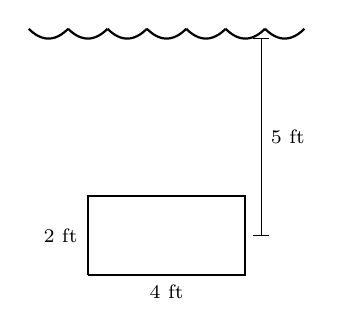
\begin{tikzpicture}[xscale=.5,yscale=.5]			
\draw [thick] (-2,-1) -- node [below,pos=.5] {\scriptsize 4 ft} (2,-1) -- (2,1) -- (-2,1) -- node [left,pos=.5] {\scriptsize 2 ft} (-2,-1);

\foreach \x in {-3,-2,-1,0,1,2,3}
{%
		\begin{scope}[shift={(\x*1,5)}]		
		\draw [thick] (-.5,.25) parabola bend (0,0) (.5,.25);
		\end{scope}
}

\draw (2.2,5) -- (2.6,5)
			(2.2,0) -- (2.6,0)
			(2.4,5) -- node [pos=.5,right] {\scriptsize 5 ft} (2.4,0);			
\end{tikzpicture}
\end{minipage}
}
{2496 lb
}
